% !TEX program=lualatex
\RequirePackage{luatex85}
\documentclass{article}
\usepackage{amsmath}
\usepackage[letterpaper,margin=1in]{geometry}
\usepackage{url}
\usepackage{graphicx}
\usepackage[utf8]{inputenc}
\usepackage[T1]{fontenc}
\usepackage[style=nature, citestyle=authoryear]{biblatex}
\usepackage{tikz}
\usepackage{wrapfig}
\usepackage{lineno}
\usepackage{outline}
\bibliography{citations.bib}
\graphicspath{./figures/}

\begin{document}
\linenumbers
\begin{outline}
	\item Introduction
	\begin{outline}
		\item What are quality scores and why are they important? \parencite{ewing_base-calling_1998} \parencite{ewing_base-calling_1998-1}
		\begin{outline}
			\item $-10\log_{10}P(e)$ \parencite{ewing_base-calling_1998} \parencite{ewing_base-calling_1998-1}
			\item Variant calling models use quality scores to weight the observed data. Generally, these models attempt to find the sample genotype most consistent with the observed data and recognize that low quality bases provide little evidence for one genotype over another. The BCFTools multiallelic caller \parencite{li_sequence_2009}, GATK's HaplotypeCaller \parencite{poplin_scaling_2018}, and FreeBayes \parencite{garrison_haplotype-based_2012} all take quality score into consideration when calling variants.
		\end{outline}
		\item What is Base Quality Score Recalibration?
		\begin{outline}
			\item Base quality scores are exactly defined as a probability. They can be interpreted as a prediction giving the probability the reported base is an error. In general, probabilities are called \textit{calibrated} if the reported probability accurately predicts the frequency of an event.
			\item Base quality scores in Illumina sequencing reads are not well-calibrated \parencite{callahan_dada2:_2016}. (TODO: more cites)
			\item Since base quality scores are used by variant calling methods, poorly calibrated reads have the potential to reduce the quality of resulting variant calls.
		\end{outline}
		\item How much does BQSR help?
		\begin{outline}
			\item BQSR improves quality score calibration in many cases.
			\item BQSR is recommended in GATK's Best Practices, but its affect on the resulting variant calls is not well-characterized.
			\begin{outline}
				\item However, \cite{ni_improvement_2016} find that improved quality score calibration aids detection of minor alleles in high coverage datasets by increasing sensitivity and reducing the number of false positive calls.
			\end{outline}
			\item BQSR is recommended for use in cancer variant discovery as well \parencite{cibulskis_sensitive_2013}, but the cancer genome is likely much different than the human genome and the database of variable sites will likely miss many sites. (TODO: find some citations)
		\end{outline}
		\item BQSR is probably most helpful with low or inconsistent coverage, as one may expect when sequencing a non-model organism; however, by definition that means you lack a quality reference and database of variable sites required for BQSR.
			\begin{outline}
				\item Find some estimates of differences between reference and samples sequenced; perhaps look at mouse
				\item This will be highly species-dependent and situation specific
			\end{outline}
		\item GATK BQSR occurs in two phases.
			\begin{outline}
				\item GATK BQSR is the most popular method for BQSR and is recommended by the GATK best practices.
				\item Phase 1 - Count errors and covariates
				\item Phase 2 - Train a hierarchical model.
				\item Phase 3 - Apply model to adjust quality score.
			\end{outline}
		\item Alternative Approaches
			\begin{outline}
			\item Alternative approaches have been developed to avoid providing a database of variable sites. However, these approaches still require a reference and alignment.
			\item Lacer \parencite{chung_lacer:_2017} bins aligned bases based on depth and whether the base matches the reference, then uses singular value decomposition to infer the shift in quality score for each base.
			\item ReQON \parencite{cabanski_reqon:_2012}, like GATK, considers bases that do not match the reference as errors but limits the number of acceptable errors at a position to minimize the effect of unknown variants. It then uses a logistic regression to recalibrate the quality scores.
			\item SOAP2 \parencite{li_soap2:_2009} is an aligner that performs BQSR during alignment (TODO: more detail)
			\item Alternative approaches use synthetic spike-ins of known composition and GATK's method \parencite{zook_synthetic_2012} or piecewise regression \parencite{ni_improvement_2016} to recalibrate quality scores. Since the sequence of the spike-in is known before hand, errors are easy to identify as there should be no biological variation in the spiked-in sample.
			\end{outline}
		\item Here we present \texttt{kbbq}, a method to recalibrate quality scores of whole genome sequencing data without a reference or database of variable sites.
	\end{outline}
	\item Methods \& Results
	\begin{outline}
		\item \texttt{kbbq} performs BQSR by adjusting how errors in the dataset are discovered.
		\begin{outline}
			\item Instead of looking at the reference, \texttt{kbbq} implements the error-correction algorithm described in \cite{song_lighter_2014} and uses the errors detected by that procedure to train and apply the standard GATK model.
			\item Briefly, the algorithm subsamples k-mers from the dataset. Since erroneous k-mers are expected to be unique, erroneous k-mers are less likely to be sampled than error-free k-mers. A binomial test is then conducted for every nucleotide in the dataset; if a sufficient number of k-mers that contain the nucleotide, the base is likely not erroneous. If \textit{k} of these bases appear next to each other, that k-mer is stored as trusted. Once the trusted k-mers have all been stored, the dataset is iterated through one last time and any non-trusted k-mers are converted to the trusted k-mer that produces the maximal number of trusted k-mers in the read. These changes are marked as errors and used to train the model.
			\item The model training and recalibration procedure are the same as those described above for GATK's BQSR method.
		\end{outline}
		\item Simulate false positives in database of variable sites and summarize degree of miscalibration (brier score and RMSE)
		\begin{outline}
			\item \includegraphics[width = 5in]{./figures/fpr.pdf}
			\item Base quality score calibration for a range of false positives in the database of variable sites. The false negative rate is zero. Increasing the false positive rate does not significantly impact the quality of the calibration.
		\end{outline}
		\item Simulate false negatives in database of variable sites and summarize degree of miscalibration (brier score and RMSE)
		% \begin{figure}[h]
		\begin{outline}
			\item 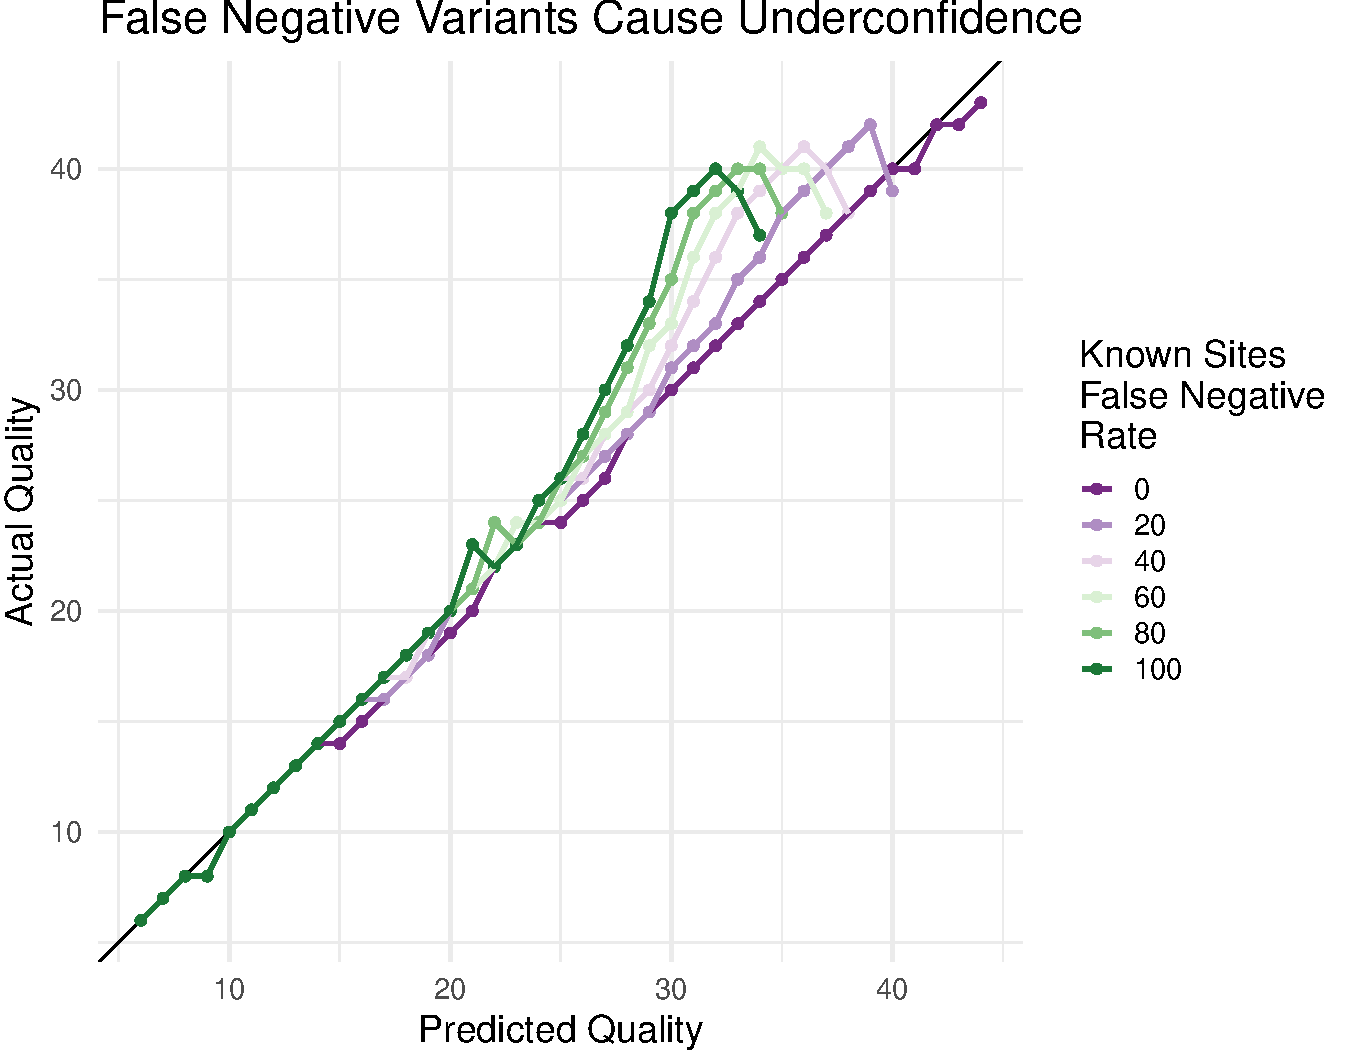
\includegraphics[width=5in]{./figures/fnr.pdf}
			\item Base quality score calibration for a range of false negatives in the database of variable sites. The false positive rate is zero. Increasing the false negative rate decreases the quality of the calibration.
			% \caption{Base quality score calibration for a range of false negatives in the database of variable sites. The false positive rate is zero. Increasing the false negative rate decreases the quality of the calibration.}
		% \end{figure}
		\end{outline}	
		\item Simulate both false positives and negatives and summarize degree of miscalibration.
		% \item Simulate downstream effect of FP and FN on variant quality; perhaps can do this with F-score - this should be done for CH3
		% \item Perhaps look at depth vs. variant quality to see if BQSR helps more in low-coverage scenarios - this should be done for CH3
		\item kbbq description
		\item application
	\end{outline}
	\item Discussion
	\begin{outline}
		\item BQSR can cause miscalibration worse than using raw data in some situations
		\item BQSR is useful in some scenarios
		\item \texttt{kbbq} is resilient to misspecified references and missing databases of variable sites, since it doesn't use those as input.
		\item Compare simulated scenarios to non-model and cancer scenarios.
		\begin{outline}
			\item In situations where the sample may not closely match the reference, use \texttt{kbbq} or don't recalibrate.
		\end{outline}
	\end{outline}
\end{outline}
\end{document}
